\documentclass[compress,violet,10pt]{beamer}

\mode<presentation>
\usetheme{Warsaw}

\usepackage{multicol}
\usepackage{amsmath}
\usepackage{caption}
\usepackage{amssymb}
\usepackage{multirow}
\usepackage[numbers]{natbib}
\usepackage{framed}
\usepackage{booktabs}
\usepackage{amsfonts}
\usepackage{hyperref}
\usepackage{ulem}
\usepackage{graphics} % for including figures
\usepackage{graphicx} % for including figures
\usepackage[update,prepend]{epstopdf} % for including eps in pdf
\def\pdfshellescape{1} % for auto converting eps to pdf
\graphicspath{{../img/}}
\newcommand*\rfrac[2]{{}^{#1}\!/_{#2}}
\newcommand{\traindata}{\ensuremath{\mathcal{T}}}
\newcommand{\matD}{\ensuremath{\mathrm{D}} }

\useoutertheme[subsection=false]{smoothbars}
\setbeamertemplate{caption}[numbered]
\setbeamercovered{transparent}

\title{Decompositional Semantics for Improved Language Models}

\author[Pranjal Singh]
{\textbf{Pranjal Singh}\\ {\small Supervisor: Dr. Amitabha Mukerjee}}
\date{June 15, 2015}

\institute{\vspace{2mm} 
B.Tech - M.Tech Dual Degree\\
\vspace{.2cm}Thesis Defense\\
\vspace{.2cm}Department of Computer Science \& Engineering\\ IIT Kanpur\\
\vspace{-2mm}
\begin{figure}[ht]
\begin{center}

\includegraphics[width=1.75cm]{iitk_logo-eps-converted-to.pdf}
\end{center}
\end{figure}
}

\AtBeginSection[]
{
	\frame{\frametitle{Outline}
    \tableofcontents[currentsection]
  }
}

\begin{document}

\frame[plain]{\frametitle{} \titlepage}
\frame{\frametitle{Outline}
  \tableofcontents
}
%===========================================================================
\section{Introduction}
\subsection{}
% -------------------------------------slide--------------------------------

\frame{\frametitle{Introduction to Decompositional Semantics}
\onslide<1->{\begin{center}
	\emph{Decompositional Semantics} is a way to describe a language entity word/paragraph/document by a constrained representation that identifies the most relevant representation conveying the semantics of the whole.\vfill
	For example, a document can be broken into aspects such as its tf-idf representation, distributed semantics vector, etc.
	\end{center}
}
}
% -------------------------------------slide--------------------------------
\frame{\frametitle{Introduction to Decompositional Semantics}
	\onslide<1->{
	\textbf{Why need Decompositional Semantics?}
	\begin{itemize}
	\vfill\item<1-> It is language independent
	\vfill\item<1-> It decomposes language entity into various aspects that are latent in its meaning
	\vfill\item<1-> All aspects are important in their own ways
\end{itemize}
}
}
% -------------------------------------slide--------------------------------
\frame{\frametitle{Introduction to Decompositional Semantics}
	\onslide<1->{Decompositional Semantics in Sentiment Analysis domain, }
	\begin{itemize} 
	\vfill\item<1-> A set of documents $D = \{d_{1}, \ldots, d_{|D|}\}$
	\vfill\item<1-> A set of aspects $A = \{a_{1}, \ldots, a_{|M|}\}$
	\vfill\item<1-> Training data for $n$ {\small ($n < |D|$)} documents, $\traindata = \{l_{d_{1}}, \ldots, l_{d_{n}}\}$ 
	\end{itemize}
\vfill
\onslide<1->{
	Example :
	\begin{table}[h!]
	\tabcolsep=0.1cm
	\tiny
	\begin{center}
	\begin{tabular}{c@{\hskip5mm} c c c c}
	\toprule
	\textbf{Documents}	&	\textbf{tf-idf} & \textbf{Word Vector Average} & \textbf{Document Vector} & \textbf{BOW}\\
	\cmidrule{1-1}
	\cmidrule{2-5}
	$d_{1}$ & 0 & 0 & 1 & 0\\
	$d_{2}$ & 0 & 1 & 1 & 0\\
	$d_{3}$ & 1 & 0 & 0 & 1\\
	$d_{4}$ & x & x & x & x\\
	$d_{5}$ & 1 & 1 & 1 & 1\\
	\bottomrule         
	\end{tabular}
	\end{center}
	\end{table}
}
\vfill
\onslide<1->{
Using $\traindata$, $D$ and $A$, the supervised classifier $\mathcal{C}$ learns a representation to predict sentiments of individual documents.}
}
% -------------------------------------slide--------------------------------
\frame{\frametitle{Problem Statement}
	\begin{block}{Better Language Representation}
	\begin{itemize}
		\item To highlight the vitality of Decompositional Semantics in language representation 
		\item To use Distributional Semantics for under resourced languages such as Hindi
		\item To demonstrate the effect of various parameters on language representation
	\end{itemize}
	\end{block}
}
% -------------------------------------slide--------------------------------
\frame{\frametitle{Contribution of this thesis}
	\begin{block}{Hindi}
	\begin{itemize}
	 \item Better representation of Hindi text using Distributional semantics 
	 \item Achieved state-of-the-art results for sentiment analysis on product and movie review corpus\footnotetext{Paper accepted in regICON'15}
	\end{itemize}
	\end{block}
\pause
	\begin{block}{New Corpus}
	\begin{itemize}
		 \item Released a corpus of 700 Hindi movie reviews
		 \item Largest corpus in Hindi in reviews domain
	\end{itemize}
  	\end{block}
\pause
	\begin{block}{English}
	\begin{itemize}
		 \item Proposed a more generic representation of English text
		 \item Achieved state-of-the-art results for sentiment analysis on IMDB movie reviews and Amazon electronics reviews\footnotetext{Submitted in EMNLP'15}
	\end{itemize}
  	\end{block}
}
%
%===========================================================================
\section[Background]{Background}
\subsection{}
%-------------------------------------slide---------------------------------
\frame{\frametitle{Background on Language Representation}
\vfill
\onslide<1->{
\textbf{Bag of Words(BOW) Model} }
\begin{itemize}
	\vfill\item<1-> Document $d_{i}$ represented by $v_{d_{i}} \in \mathbb{R}^{|V|}$
	\vfill\item<1-> Each element in $v_{d_{i}}$ denotes presence/absence of each word
	\vfill\item<2-> \textbf{Drawbacks}:
	\begin{itemize}
		\vfill\item<2-> High-dimensionality
		\vfill\item<2-> Ignores word ordering
		\vfill\item<2-> Ignores word context
		\vfill\item<2-> Very sparse
		\vfill\item<2-> No relative importance to words
	\end{itemize}
\end{itemize}
\vfill
}
%-------------------------------------slide---------------------------------
\frame{\frametitle{Background on Language Representation}
\vfill
\onslide<1->{
\textbf{Term Frequency-Inverse Document Frequency(tf-idf) Model} }
\begin{itemize}
	\vfill\item<1-> Document $d_{i}$ represented by $v_{d_{i}} \in \mathbb{R}^{|V|}$
	\vfill\item<1-> Each element in $v_{d_{i}}$ is the product of term frequency and inverse document frequency:$tfidf(t,d)=tf(t,d) \times \log(\frac{\|D\|}{df(t)})$
	\vfill\item<1-> Gives weights to terms which are less frequent and hence important
	\vfill\item<2-> \textbf{Drawbacks}:
	\begin{itemize}
		\vfill\item<2-> High-dimensionality
		\vfill\item<2-> Ignores word ordering
		\vfill\item<2-> Ignores word context
		\vfill\item<2-> Very sparse
		\vfill\item<2-> \sout{No relative importance to words}
	\end{itemize}
\end{itemize}
\vfill
}
%-------------------------------------slide---------------------------------
\frame{\frametitle{Background on Language Representation}
\vfill
\onslide<1->{
\textbf{Distributed Representation of Words(Mikolov et al., 2013b)}}
\begin{itemize}
	\vfill\item<1-> Each word $w_{i} \in V$ is represented using a vector $v_{w_i} \in \mathbb{R}^{k}$
	\vfill\item<1-> The vocabulary $V$ can be represented by a matrix $V \in \mathbb{R}^{k \times |V|}$
 	\vfill\item<1->	Vectors ($v_{w_{i}}$) should encode the semantics of the words in vocabulary
	\vfill\item<2-> \textbf{Drawbacks}:
	\begin{itemize}
		\vfill\item<2-> Ignores exact word ordering
		\vfill\item<2-> Cannot represent documents as vectors without \emph{composition}
	\end{itemize}
\end{itemize}
\vfill
}
%-------------------------------------slide---------------------------------
\frame{\frametitle{Background on Language Representation}
\vfill
\onslide<1->{
\textbf{Distributed Representation of Documents(Le and Mikolov, 2014)}}
\begin{itemize}
	\vfill\item<1-> Each document $d_{i} \in D$ is represented using a vector $v_{d_i} \in \mathbb{R}^{k}$
	\vfill\item<1-> The set $D$ can be represented by a matrix $D \in \mathbb{R}^{k \times |D|}$
 	\vfill\item<1->	Vectors ($v_{d_{i}}$) should encode the semantics of the documents
	\vfill\item<2-> \textbf{Comments}:
	\begin{itemize}
		\vfill\item<2-> Can represent documents
		\vfill\item<2-> Ignores contribution of indvidual word while building document vectors
	\end{itemize}
\end{itemize}
\vfill
}
%-------------------------------------slide---------------------------------
\frame{\frametitle{Background on Sentiment Analysis}
\vfill
\begin{itemize}
	\vfill\item<1-> Pang et al.(2004) obtained 87.2\% accuracy on a dataset that discarded objective sentences and used text categorization techniques on the subjective sentences
	\vfill\item<1-> Socher et al.(2013) used recursive neural network over sentiment treebank for sentiment classification
	\vfill\item<1-> Le and Mikolov (2014) use document vector model and obtained 92.6\% accuracy on IMDB movie review dataset
\end{itemize}
\vfill
}
%-------------------------------------slide---------------------------------
\frame{\frametitle{Background on Sentiment Analysis}
\vfill
\onslide<1->{There has been limited work on sentiment analysis in Hindi}
\begin{itemize}
	\vfill\item<2-> Joshi et al.(2010) used In-language sentiment analysis, Machine Translation and Resource Based Sentiment Analysis to achieve 78.1\% accuracy
	\vfill\item<2-> Mukherjee et al.(2012) presented the inclusion of discourse markers in a BOW model to improve the sentiment classification accuracy by 2-4\%
	\vfill\item<2-> Mittal et al.(2013) incorporate hand-coded rules dealing with negation and discourse relations achieving 80.2\% accuracy
\end{itemize}
\vfill
}

%===========================================================================
\section[Datasets]{Datasets}
\subsection{}
%-------------------------------------slide---------------------------------
\frame{\frametitle{Hindi Product and Movie Review Corpus}
\vfill
\begin{itemize}
	\vfill\item<1-> Product Review dataset (LTG, IIIT Hyderabad) contains 350 Positive reviews and 350 Negative reviews
	\vfill\item<1-> Movie Review dataset (CFILT, IIT Bombay) contains 127 Positive reviews and 125 Negative reviews
	\vfill\item<1-> Each review is around 1-2 sentences long and the sentences are mainly focused on sentiment, either positive or negative.
\end{itemize}
\vfill
}
%-------------------------------------slide---------------------------------
\frame{\frametitle{700-Movie Review Corpus}
\vfill
\begin{itemize}
	\vfill\item<1-> We collected Hindi movie reviews from websites such as \emph{Dainik Jagran} and \emph{Navbharat Times}
	\vfill\item<1-> The movie reviews are longer than the previous corpus and contains subjects other than sentiment
\end{itemize}
\begin {table}[h!]
\centering
\begin{tabular}{ |l|l| }
\hline
\multicolumn{2}{|c|}{\textbf{Overall}} \\
\hline
Positive Reviews & 356 \\ 
Negative Reviews & 341 \\
Total Reviews & 697\\ \hline
\multicolumn{2}{|c|}{29.7 sentences per document} \\ \hline
\multicolumn{2}{|c|}{494.6 words per document} \\
\hline
\end{tabular}
\caption {Statistics of Movie Reviews from Jagran and Navbharat}
\end{table}
\vfill
}
%-------------------------------------slide---------------------------------
\frame{\frametitle{English Corpus}
\vfill
	\begin{block}{IMDB Movie Reviews}
	\begin{itemize}
	 \item Contains 25,000 positive and 25,000 negative reviews for training purpose
	 \item It also contains an additional 50,000 unlabeled documents for unsupervised learning
	\end{itemize}
	\end{block}
	\begin{block}{Amazon Product Reviews}
	\begin{itemize}
	 \item There are 3 review datasets: Watches, Electronics and MP3 each of size 30.8MB, 728.4MB and 27.7MB respectively
	 \item Electronics dataset consists of 1,241,778 reviews, Watches Dataset consists of 68,356 reviews and MP3 Dataset consists of 31,000 reviews
	 \item Datasets are split into 80-20 ratio for training and testing
	\end{itemize}
	\end{block}
\vfill
}
%-------------------------------------slide---------------------------------
\frame{\frametitle{Wikipedia}
\vfill
	\begin{block}{Hindi}
		Hindi Wikipedia text dump (approx. 290MB) containing around 24M words with 724K words in the vocabulary.
	\end{block}
	\begin{block}{English}
		English Wikipedia text dump (approx. 20.3GB) contains around 3.5B words with 7.8M words in the vocabulary.
	\end{block}
\vfill
}
%===========================================================================
\section[Method and Experiments]{Method and Experiments}
\subsection{}

%-------------------------------------slide---------------------------------
\frame{\frametitle{Distributed Word Representation}
\vfill
\onslide<1->{\textbf{Skipgram}}
\begin{itemize}
	\vfill\item<1-> Each current word acts as an input to a log-linear classifier with continuous projection layer, and predict words within a certain range before and after the current word
	\vfill\item<1-> The objective is to maximize the probability of the context given a word:
	\begin{center}
	$p(c|w;\theta)=\frac{\exp^{v_c.v_w}}{\sum_{c' \in C}\exp^{v_c.v_w}}$
	\end{center}
	\vfill\item<1-> $v_c$ and $v_w$ $\in$ $R^d$ are vector representations for context $c$ and word $w$ respectively. $C$ is the set of all available contexts. The parameters $\theta$ are $v_{c_i}$, $v_{w_i}$ for $w \in V$, $c \in C$, $i \in 1,....,d$ 
\end{itemize}
\vfill
}
%-------------------------------------slide---------------------------------
\frame{\frametitle{Distributed Word Representation}
\vfill
\begin{itemize}
	\vfill\item<1-> Weights between the input layer and the output layer can be represented by a $V \times N$ matrix \textbf{W}
	\vfill\item<1-> Each row of \textbf{W} is the $N$-dimension vector representation $v_w$ of the associated word of the input layer
	\vfill\item<-1> Given a word, assuming $x_k=1$ and $x_{k'}=0$ for $k' \neq k$, then
	\begin{center}
	$h=x^TW=W_{(k,.)}:=v_{w_I}$\\
	$u_j={v'}_{w_j}^T.h$
	\end{center}
	\vfill\item<-1> $v_{w_I}$ is the vector representation of the input word $w_I$ and $u_j$ is the score of each word in the vocabulary
	\vfill\item<1-> There is a different weight matrix \textbf{W'}=$\{w_{ij}^{'}\}$ which is a $N \times V$ matrix between hidden and output layer
	\vfill\item<1-> Softmax function is used to predict probabilities and Stochastic Gradient Descent is used to update the parameters of the model
\end{itemize}
\vfill
}
%-------------------------------------slide---------------------------------
\frame{\frametitle{Distributed Document Representation}
\vfill
	\begin{block}{Motivation}
	\begin{itemize}
	 \item Drawbacks in BOW like sparsity, high-dimensionality, inability to encode context information and consider word ordering
	 \item Composition models alone cannot represent documents (Blacoe and Lapata, 2012)
	 \item Recursive Tensor Neural Networks (Socher et al.,2013) are computationally expensive and cannot be composed into document vectors when there are multiple sentences due to parsing issues
	 \item Presence of similarity measures to deal with synonyms or semantically similar documents 
	\end{itemize}
	\end{block}
\vfill
}
%-------------------------------------slide---------------------------------
%\frame{\frametitle{Distributed Document Representation}
%\vfill
%\begin{itemize}
%	\vfill\item<1-> Every document is now mapped to a unique vector and id, represented by a matrix $D$
%	\vfill\item<1-> Word vector matrix $W$ is shared across all documents and contexts are now separately sampled for each document
%	\vfill\item<1-> The only difference in this model is that $h$ is now constructed with both $W$ and $D$.
%\end{itemize}
%\vfill
%}
%-------------------------------------slide---------------------------------
\frame{\frametitle{Semantic Composition}
\vfill
\onslide<1->{
The \emph{Principle of Compositionality} is that meaning of a complex expression is determined by the meaning of its constituents and the rules which guide this combination. It is also known as \emph{Frege's Principle}.\\ For example,
\begin{center}
\emph{The movie is funny and the screenplay is good}
\end{center}
In the above sentence, consider the word vectors are represented by $w(x)$ and the sentence vector as $S(x)$. Hence,
\begin{align}
S(x) = c_1w_1(x) \Theta c_2w_2(x) \Theta c_3w_3(x) \Theta c_4w_4(x) \dots \Theta c_kw_k(x)
\end{align}
where $\Theta$ can be any operation(e.g., addition, multiplication) and $c_i$s are constants.}
\vfill
}
%-------------------------------------slide---------------------------------
\frame{\frametitle{Semantic Composition}
\vfill
\begin{itemize}
\vfill\item<1-> We describe two approaches to incorporate graded weighting into word vectors for building document vectors.\\
\vfill\item<2-> Let $v_{w_i}$ be the vector representation of the $i^{th}$ word. Then document vector $v_{d_i}$ for $i^{th}$ document is:
$$
v_{d_i} = \left\{
        \begin{array}{ll}
            0 & \quad w_k \in stopwords \\
            \sum\limits_{w_k \in d_i} v_{w_k} & \quad w_k \notin stopwords
        \end{array}
    \right.
$$
The above equation is 0-1 step-function which ignores contribution of all stop words.
\vfill\item<3-> Another schema which incorporates \emph{idf} weight is:
$$
v_{d_i} = \left\{
        \begin{array}{ll}
            0 & \quad idf(w_k,d_i) \leq \delta \\
            \sum\limits_{w_k \in d_i} idf(w_k,d_i).v_{w_k} & \quad otherwise
        \end{array}
    \right.
$$
where $\delta$ is a pre-defined threshold below which the word has no importance and above which the \emph{idf} terms gives importance to that particular word.
\end{itemize}
\vfill
}
%-------------------------------------slide---------------------------------
\frame{\frametitle{Semantic Composition}
\vfill
\begin {table}[h!]
	\centering
	\begin{tabular}{ |c|c| }
	\hline
	Composition & Accuracy \\ \hline \hline
	Multiplication & 50.30 \\ \hline
	Average & 88.42 \\ \hline
	Weighted Average & \textbf{89.56} \\ \hline
	\end{tabular}
	\caption {Results of Vector Composition with different Operations}
	\label{table:composition}
\end{table}
\begin{table}[h]
\centering
\small
\begin{tabular}{|l|l|l|l|}
\hline
\textbf{Method}                                                                 & \textbf{Weight} & \textbf{Accuracy(1)} & \textbf{Accuracy(2)} \\ \hline
\multirow{2}{*}{\begin{tabular}[c]{@{}l@{}}0-1 \\ Weighting\end{tabular}}       & 0               & 93.84                & 93.06                \\ \cline{2-4} 
                                                                                & 1               & \textbf{93.91}       & \textbf{93.18}       \\ \hline
\multirow{5}{*}{\begin{tabular}[c]{@{}l@{}}Graded idf \\ Weighting\end{tabular}} & 2               & \textbf{93.89}       & 93.17                \\ \cline{2-4} 
                                                                                & 2.5             & 93.87                & 93.16                \\ \cline{2-4} 
                                                                                & 2.8             & 93.86                & 93.16                \\ \cline{2-4} 
                                                                                & 3               & 93.86                & \textbf{93.22}       \\ \cline{2-4} 
                                                                                & 4               & 93.83                & 93.12                \\ \hline
\end{tabular}
\caption {Results on IMDB Movie Reviews(Composite Document Vector);Accuracy(2) is when we exclude tf-idf features}
\label{table:graded_weighting_tfidf}
\end{table}
}
%-------------------------------------slide---------------------------------
\frame{\frametitle{Effect of Context Size}
\vfill
\begin{figure}
	\centering
	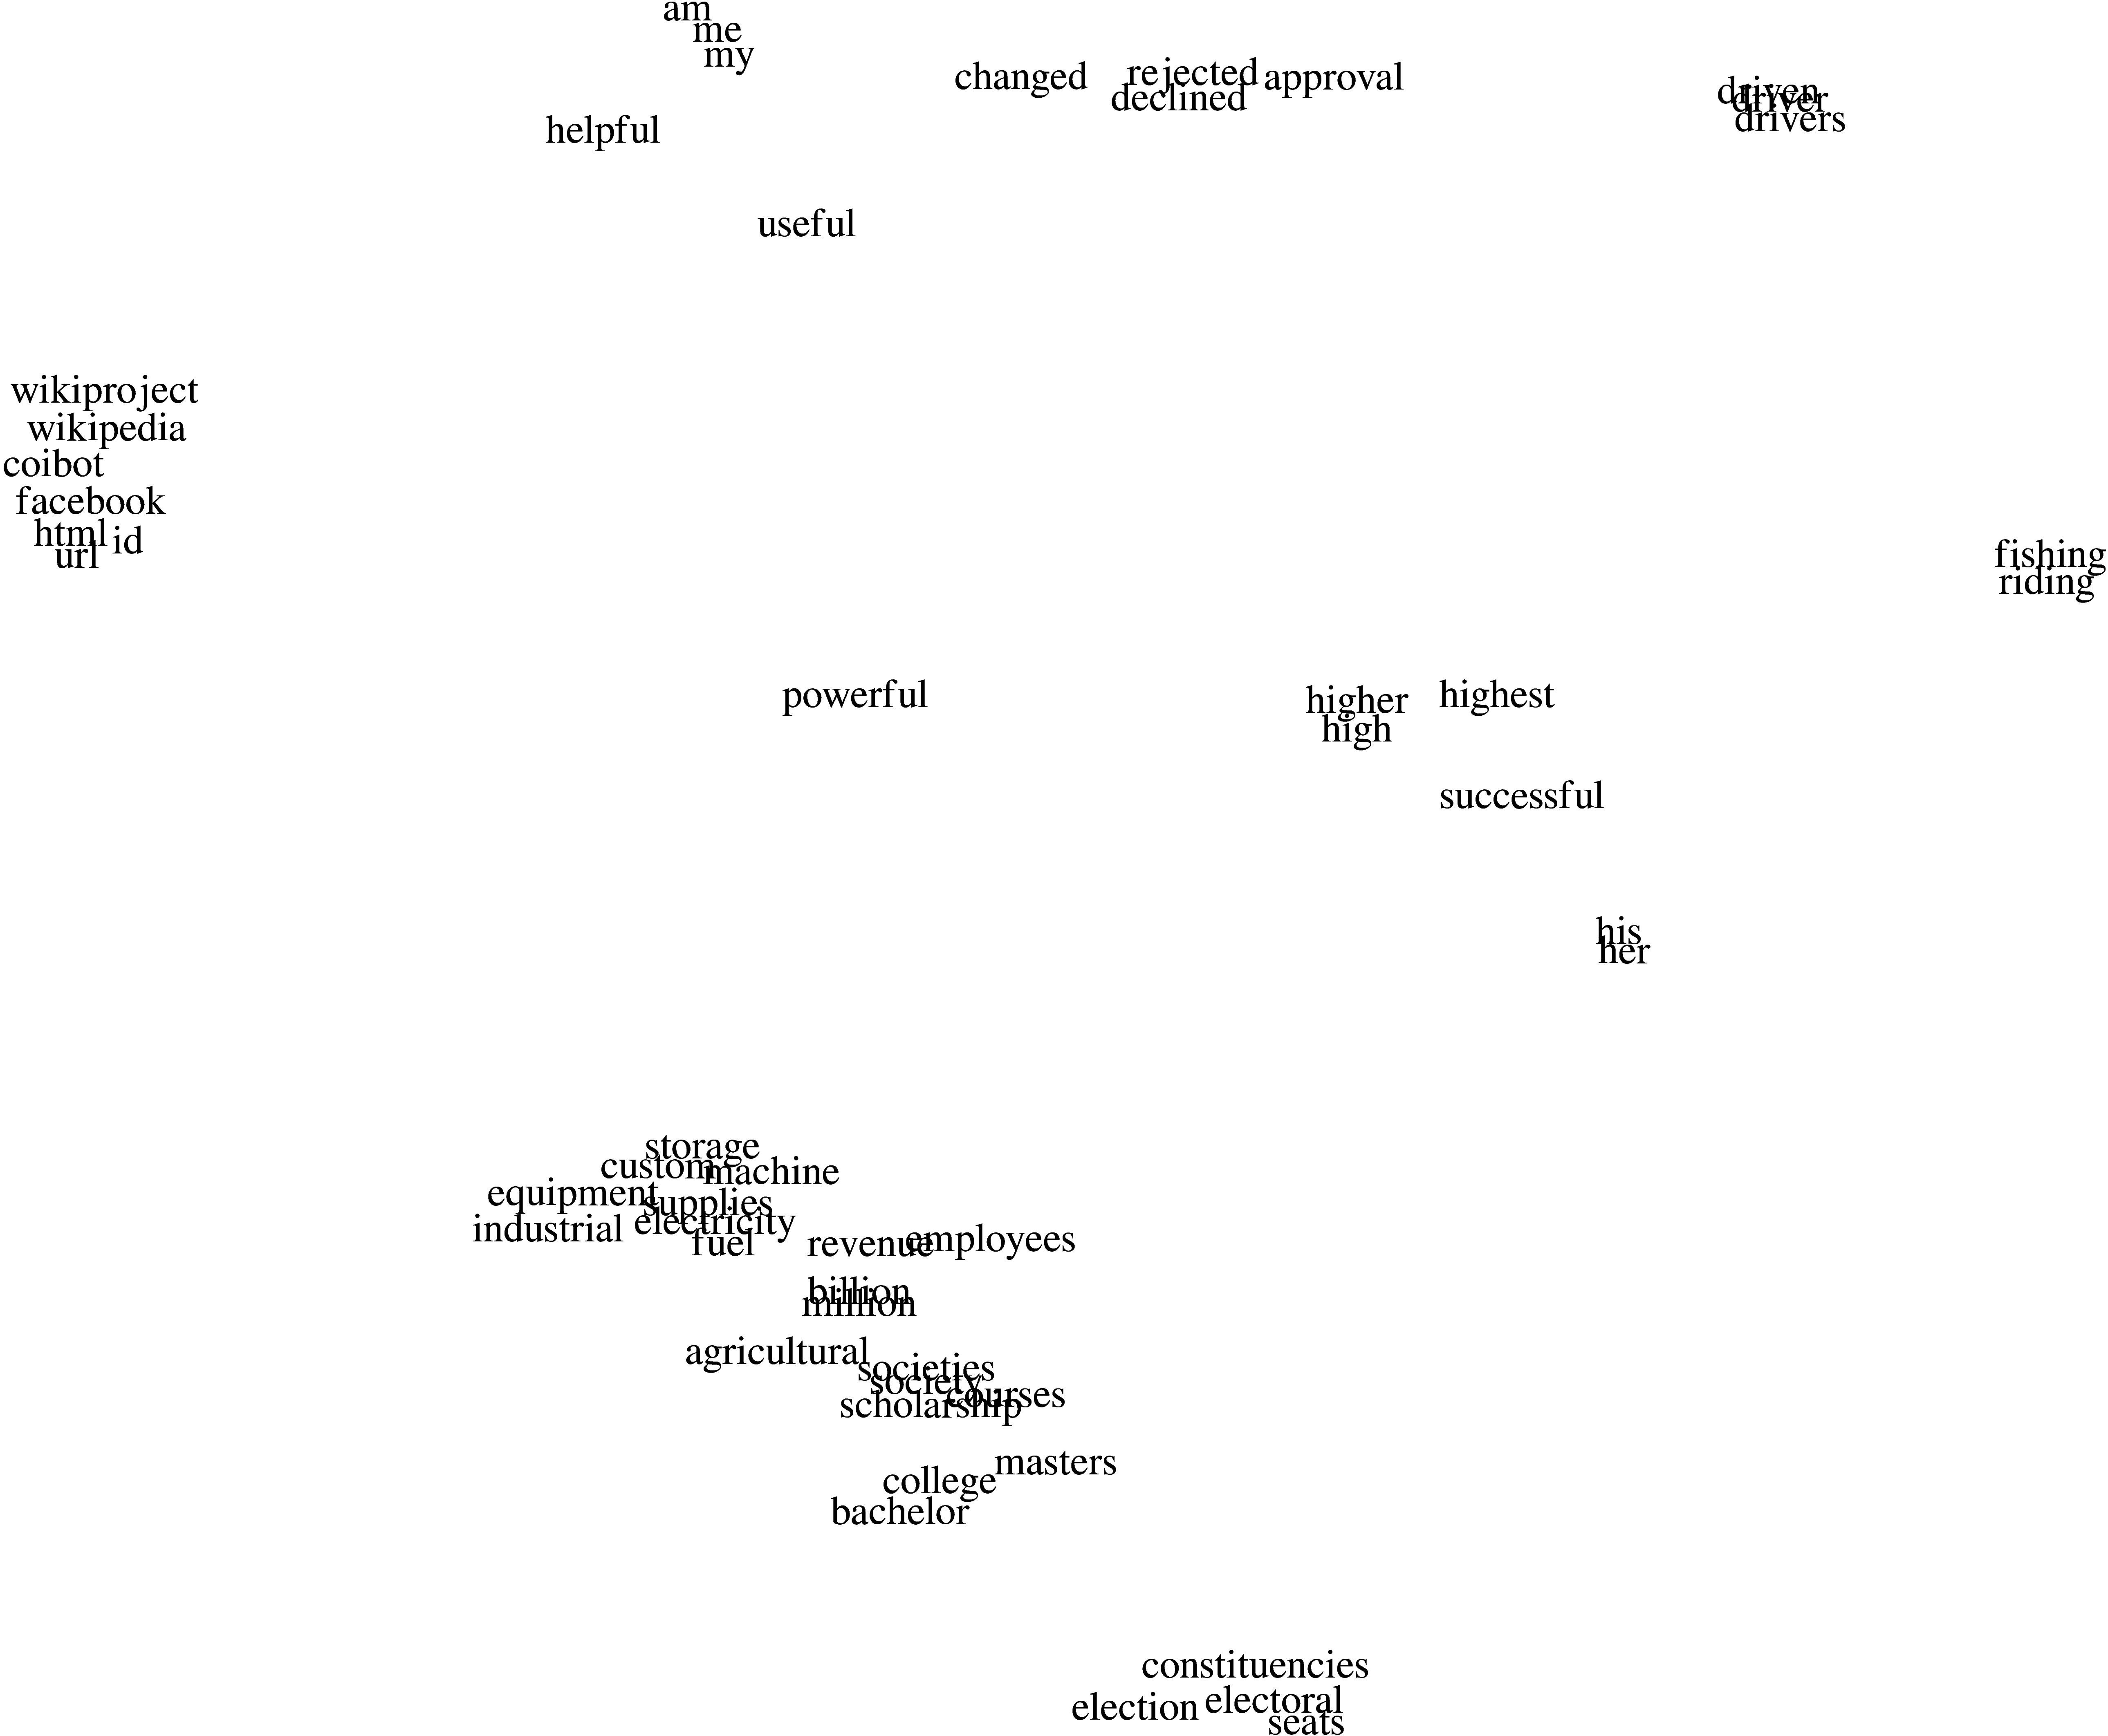
\includegraphics[scale=0.04]{../img/tsne_5.jpg}
	\caption{High Dimensional representation of Wiki Text with Context Size 5}
	\label{fig:tsne_5}
\end{figure}
\vfill
}
%-------------------------------------slide---------------------------------
\frame{\frametitle{Effect of Context Size}
\vfill
\begin{figure}
	\centering
	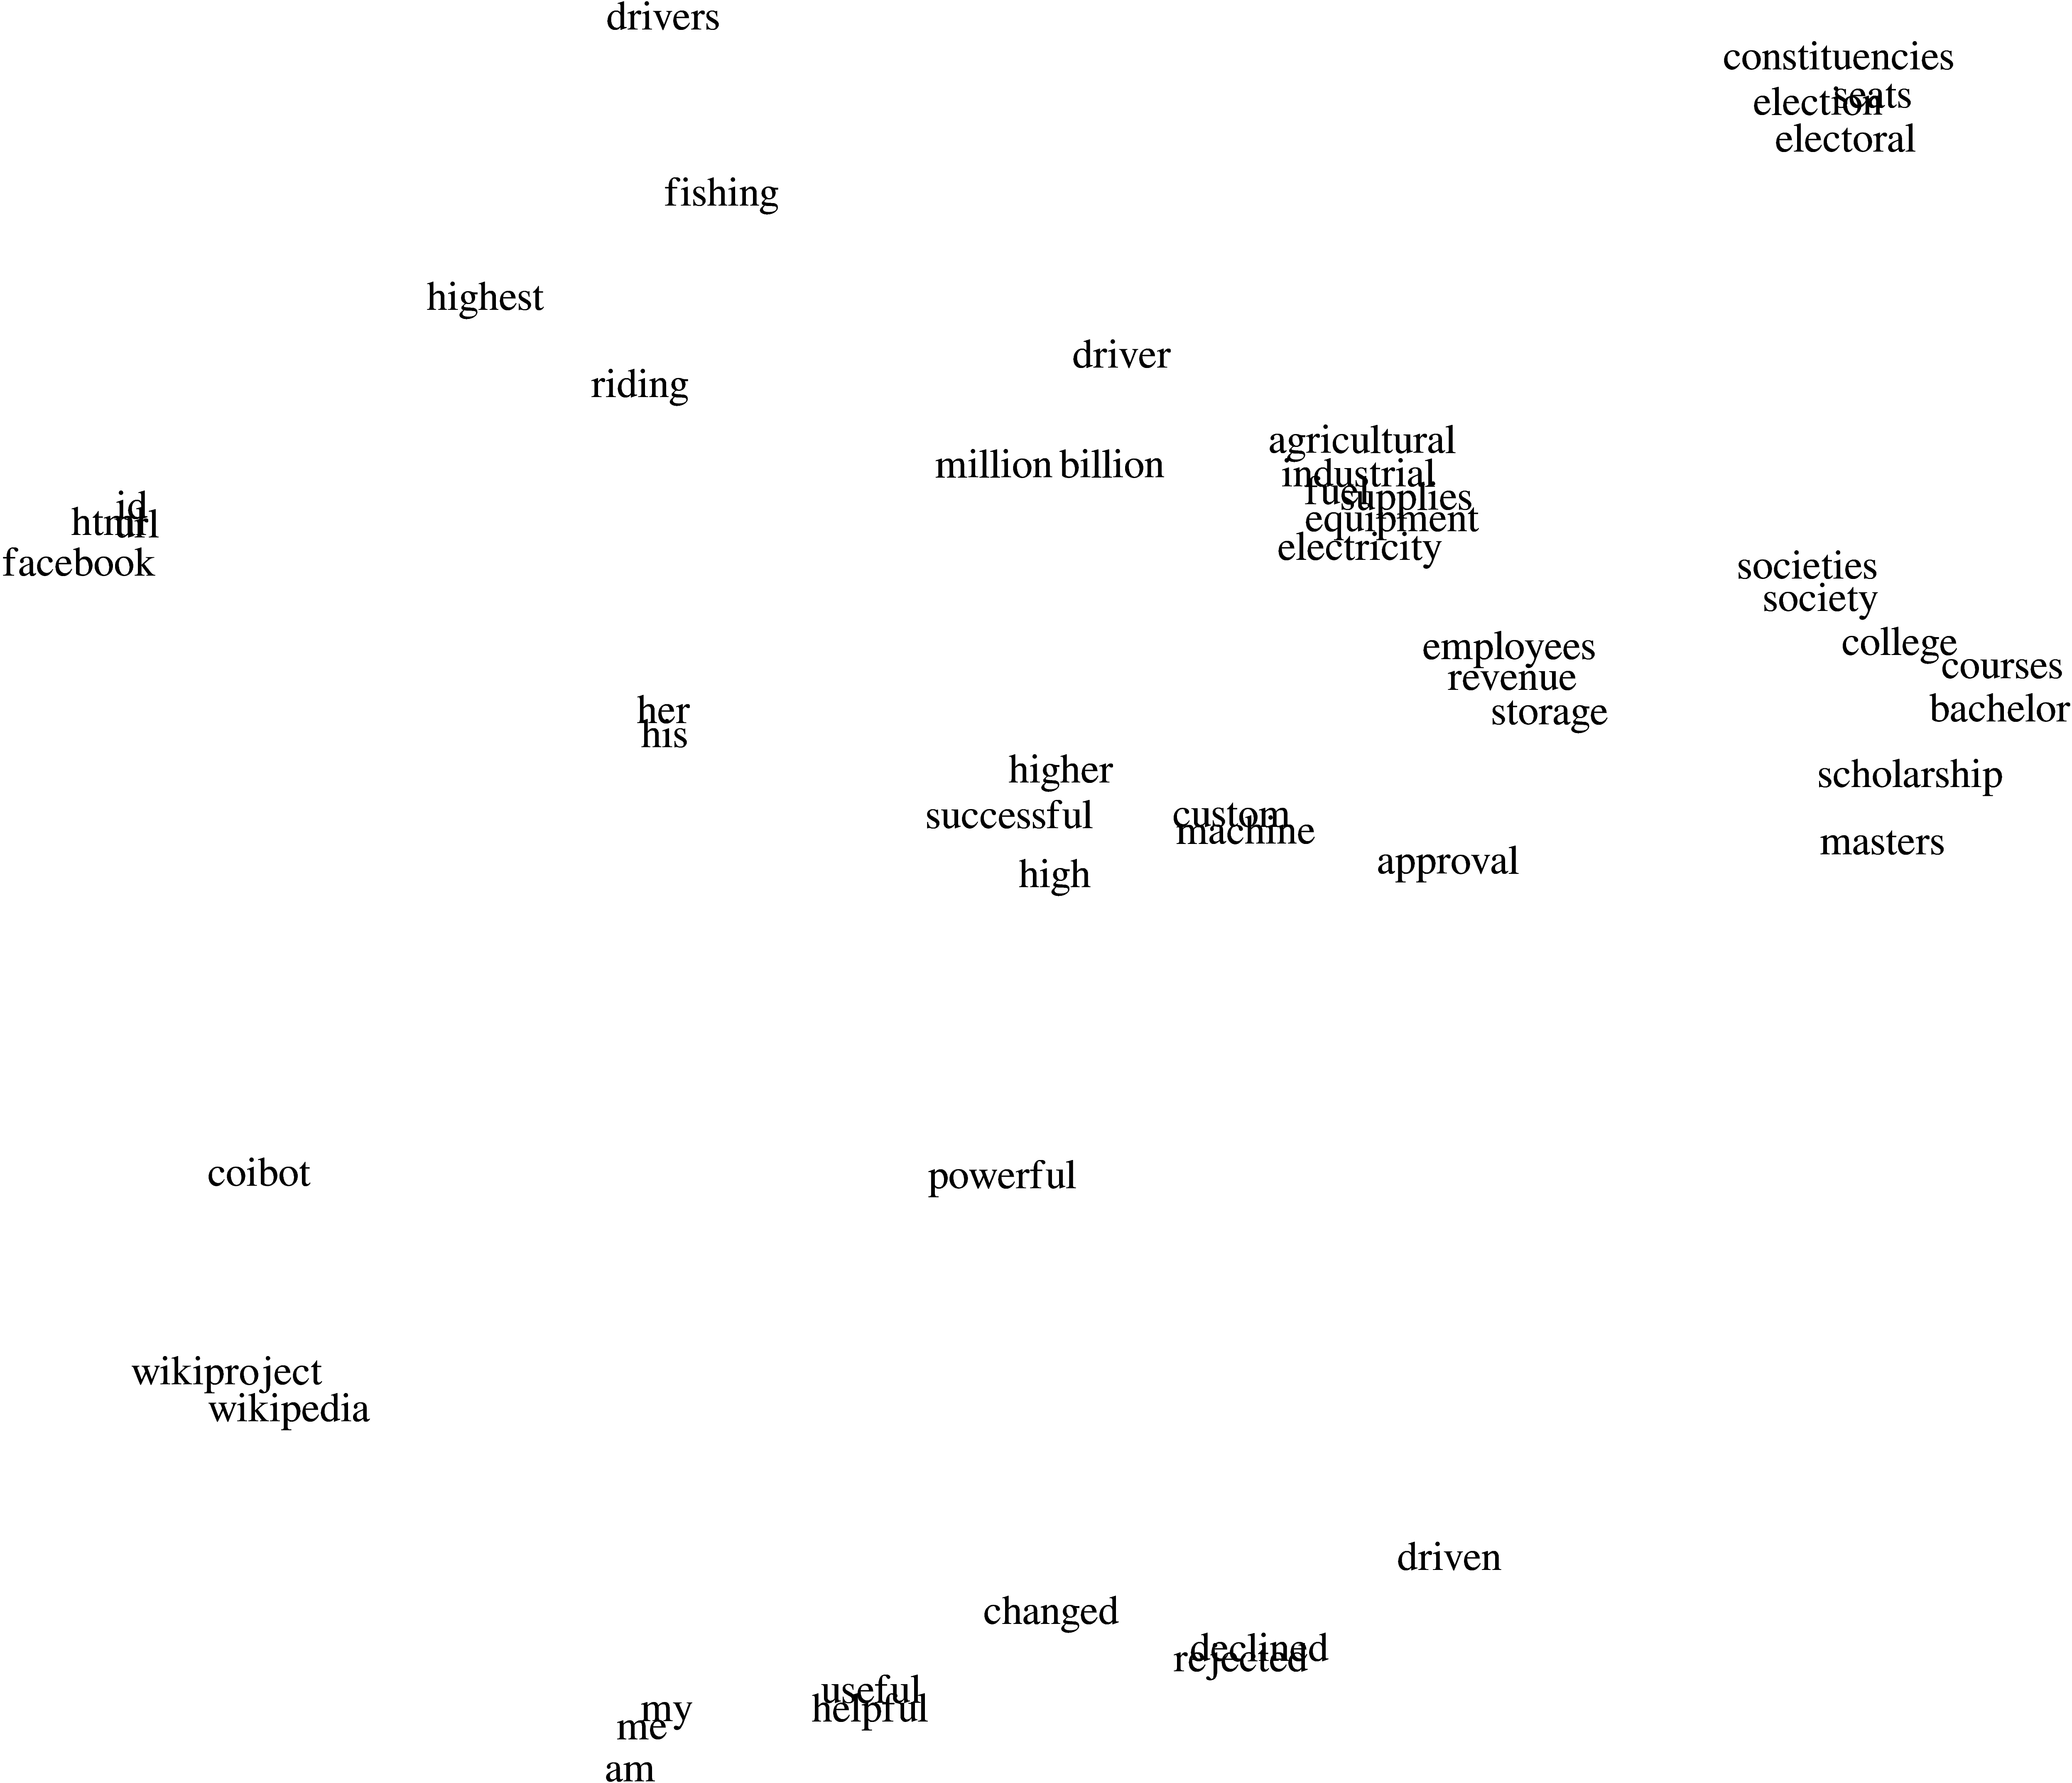
\includegraphics[scale=0.04]{../img/tsne_10.jpg}
	\caption{High Dimensional representation of Wiki Text with Context Size 10}
	\label{fig:tsne_10}
\end{figure}
\vfill
}
%-------------------------------------slide---------------------------------
\frame{\frametitle{Effect of Context Size}
\vfill
\begin{figure}
	\centering
	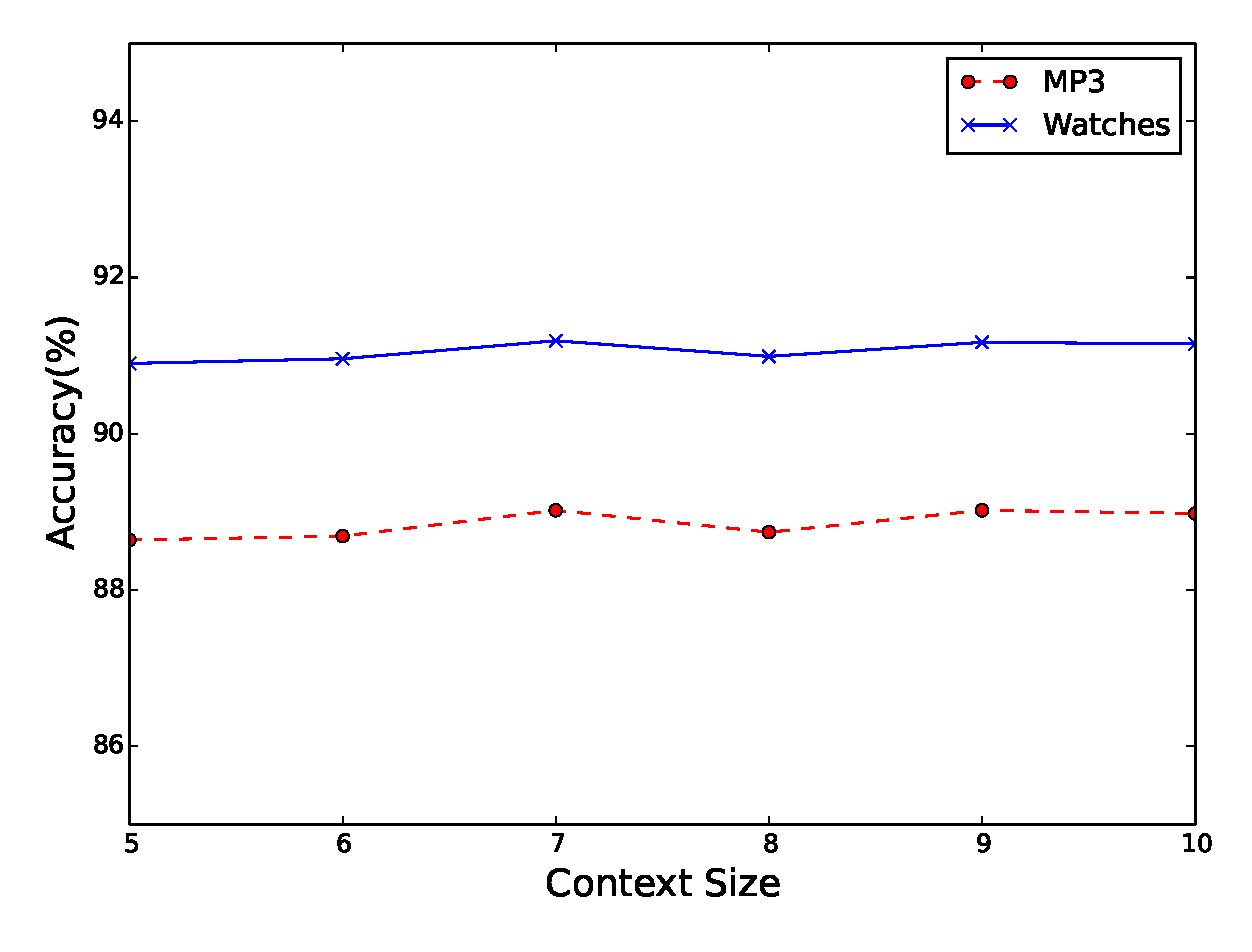
\includegraphics[scale=0.4]{../img/context_size.eps}
	\caption{Variation of Accuracy with Different Context Size on Watches and MP3 Datasets}
	\label{fig:context_size}
\end{figure}
\vfill
}
%-------------------------------------slide---------------------------------
\frame{\frametitle{SkipGram or CBOW?}
\vfill
\begin{figure}[ht!]
\centering
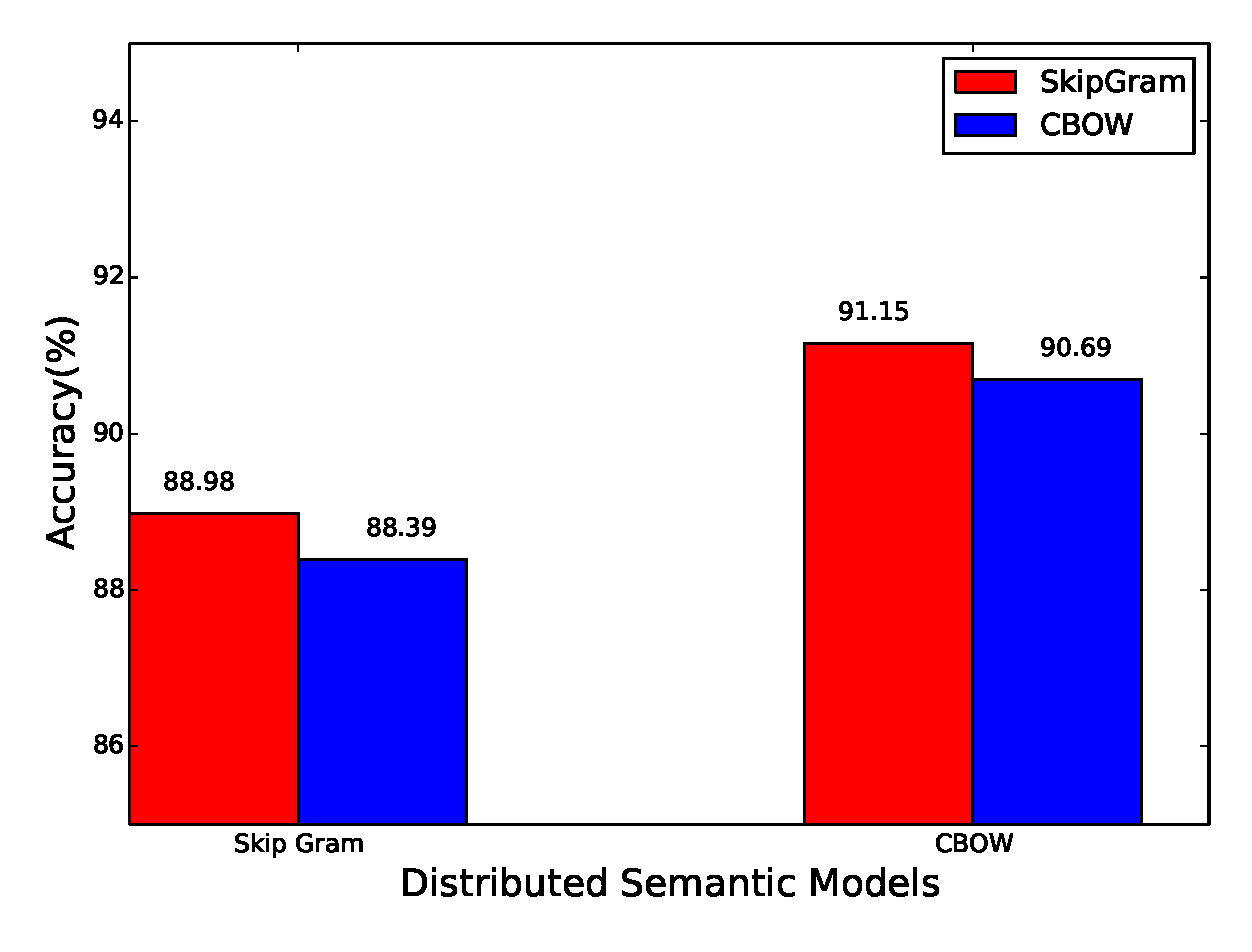
\includegraphics[scale=0.4]{accuracy_sgcbow.eps}
\caption{Variation of Accuracy with skipgram and cbow on Watches and MP3 Datasets. \label{fig:accuracy_sgcbow}}
\end{figure}
\vfill
}
%-------------------------------------slide---------------------------------
\frame{\frametitle{Work Flow}
\vfill
     \begin{figure}
	\centering
	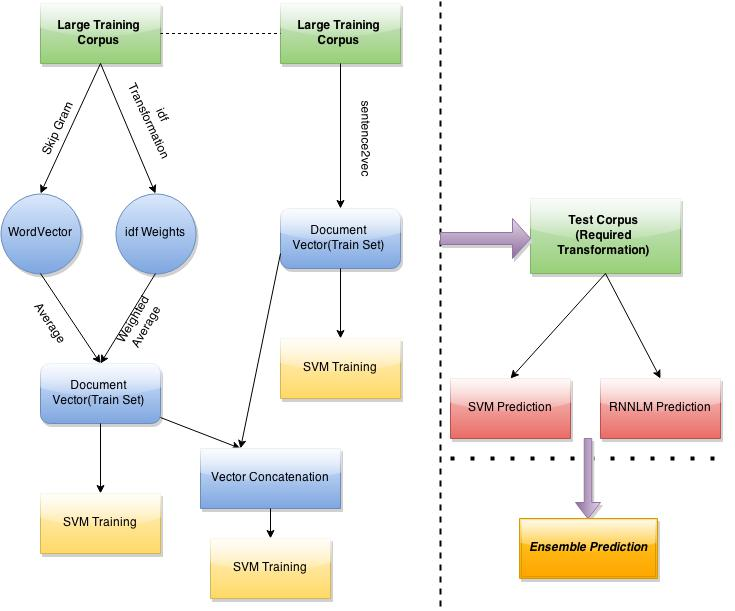
\includegraphics[scale=0.3]{../img/flow_chart.jpg}
	\caption{Work Flow}
	\label{fig:workflow}
    \end{figure}
\vfill
}

%===========================================================================
\section[Results]{Results}
\subsection{}
%-------------------------------------slide---------------------------------
\frame{\frametitle{Result on English Dataset}
\vfill
\begin{table}[h]
	\centering
	\begin{tabular}{|c|c|c|c|}
	\hline
	\textbf{Method}                                                             & \textbf{IMDB}  & \textbf{Amazon} & \textbf{Hindi} \\ \hline
	RNNLM (Baseline)                                               & 86.45          & 90.03           & 78.84          \\ \hline
	Paragraph Vector(Le and Mikolov,2014)                                               & 92.58          & 91.30           & 74.57          \\ \hline
	Averaged Vector                                                             & 88.42          & 88.52           & 79.62          \\ \hline
	Weighted Average Vector                                                            & 89.56          & 88.63               & 85.90          \\ \hline
	Composite Document Vector                                     & 93.91          & 92.17               & 90.30         \\ \hline
	\end{tabular}
	\caption {Comparison of accuracies on 3 Datasets(IMDB, Amazon Electronics Review and Hindi Movie Reviews(IITB)) for various types of document composition models. The state of the art for these tasks are: IMDB: 92.58\%; Amazon:85.90\%, Hindi:79.0\%.}
	\label{table:3Datasets}
\end{table}
\vfill
}
%-------------------------------------slide---------------------------------
\frame{\frametitle{Result on English Dataset}
\vfill
\begin{table}[h]
	\centering
	\begin{tabular}{ | c | c | }
	\hline
	\textbf{Method} & \textbf{Accuracy} \\ \hline
	Maas et al.(2011) & 88.89\\ \hline
	NBSVM-bi (Wang \& Manning, 2012) & 91.22\\ \hline
	NBSVM-uni (Wang \& Manning, 2012) & 88.29\\ \hline
	SVM-uni (Wang \& Manning, 2012) & 89.16\\ \hline
	Paragraph Vector (Le and Mikolov(2014)) & 92.58\\ \hline
	WordVector+Wiki(Our Method) & 88.60\\ \hline
	Weigted WordVector+TfIdf(Our Method) & 89.56\\ \hline
	Weighted WordVector+TfIdf+Document Vector & \textbf{93.91}\\ \hline
	Ensemble of Enhanced Document Vector and RNNLM & 94.19 \\ \hline
	\end{tabular}
	\caption {Results on IMDB Movie Review Dataset}
	\label{table:IMDB}
\end{table}
\vfill
}
%-------------------------------------slide---------------------------------
\frame{\frametitle{Result on English Dataset}
\vfill
\begin{table}[h]
	\centering
	\begin{tabular}{ | c | c | }
	\hline
	\textbf{Method} & \textbf{Accuracy} \\ \hline
	WordVector Averaging & 88.42\\ \hline
	Weighted WordVector Average & 89.56\\ \hline
	Weigted WordVector Averaging+Wiki & 88.60\\ \hline
	Weigted WordVector Averaging+TfIdf & 90.67\\ \hline
	WordVector Averaging+Document Vector & 93.18\\ \hline
	WordVector Averaging+Wiki+Document Vector & 93.18\\ \hline
	WordVector Averaging+Document Vector+RNNLM & 93.70\\ \hline
	WordVector Averaging+Wiki+Document Vector+RNNLM & 93.57\\ \hline
	WordVector Averaging+TfIdf+Document Vector & 93.91\\ \hline
	WordVector Averaging+Wiki+Document Vector+TfIdf & 93.55\\ \hline
	WordVector Averaging+TfIdf+Document Vector+RNNLM & \textbf{94.19}\\ \hline
	\end{tabular}
	\caption {Comparison of results on IMDB Movie Review Dataset with Various Features}
	\label{table:IMDB_features}
\end{table}
\vfill
}
%-------------------------------------slide---------------------------------
\frame{\frametitle{Result on English Dataset}
\vfill
\begin{figure}[H]
\centering
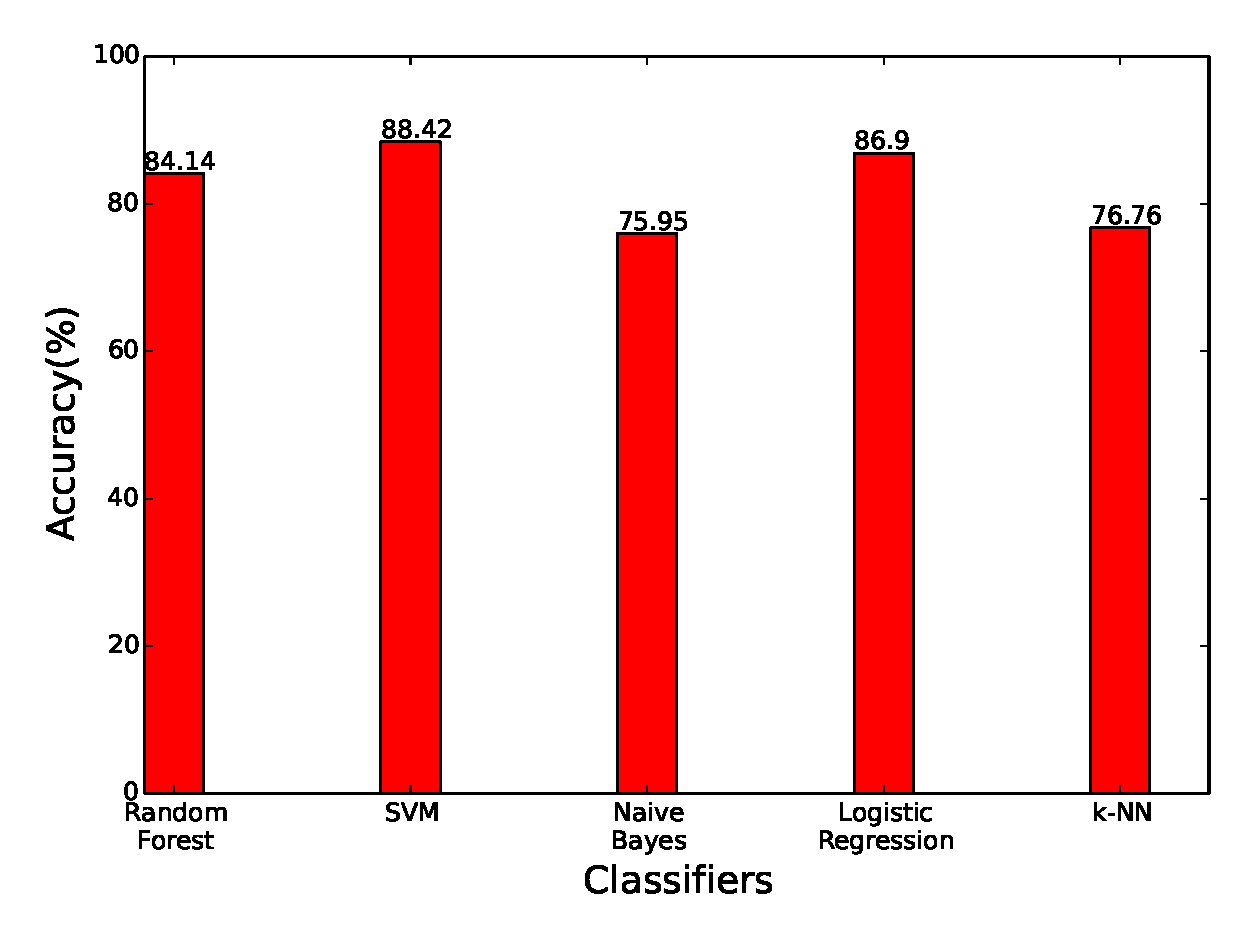
\includegraphics[scale=0.4]{accuracy_wordvectors.eps}
\caption{Accuracies of Different Classifiers with Average Word Vectors on IMDB Dataset. \label{fig:accuracy_wordvectors}}
\end{figure}
\vfill
}
%-------------------------------------slide---------------------------------
\frame{\frametitle{Result on English Dataset}
\vfill
\begin{table}[h]
	\centering
	\begin{tabular}{ | c | c | }
	\hline
	\textbf{Features} & \textbf{Accuracy} \\ \hline
	Dredze et al.(2008) & 85.90\\ \hline
	Max Entropy & 83.79\\ \hline
	WordVector Averaging (Our Method) & 89.41\\ \hline
	Composite Document Vector(Our Method) & 92.17\\ \hline
	Composite Document Vector+RNNLM & \textbf{92.91}\\ \hline
	\end{tabular}
	\caption {Results on Amazon Electronics Review Dataset}
	\label{table:amazon}
\end{table}
\vfill
}
%-------------------------------------slide---------------------------------
\frame{\frametitle{Result on Hindi Dataset}
\vfill
\begin {table}[h!]
	\centering
	\begin{tabular}{ | c | c | c | }
	\hline
	\textbf{Features} & \textbf{Accuracy(1)} & \textbf{Accuracy(2)} \\ \hline
	WordVector Averaging & 78.0 & 79.62\\ \hline
	WordVector+tf-idf & 90.73 & 89.52\\ \hline
	WordVector+tf-idf without stop words & 91.14 & 89.97\\ \hline
	Weighted WordVector & 89.71 & 85.90\\ \hline
	Weighted WordVector+tf-idf & \textbf{92.89} & \textbf{90.30}\\ \hline
	\end{tabular}
	\caption {Accuracies for Product Review and Movie Review Datasets.}
	\label{table:hindi_ourmethods}
\end{table}
\vfill
}
%-------------------------------------slide---------------------------------
\frame{\frametitle{Result on Hindi Dataset}
\vfill
\begin {table}[h!]
	\centering
	\tiny
	\begin{tabular}{ | c | c | c | }
	\hline
	\textbf{Experiment} & \textbf{Features} & \textbf{Accuracy} \\ \hline
	Subjective Lexicon (Bakliwal et al.(2012)) & Simple Scoring & 79.03\\ \hline
	Hindi-SWN Baseline (Arora et al.(2013)) & Adjective and Adverb presence & 69.30\\ \hline
	Word Vector with SVM (Our method) & tf-idf with word vector & 91.14\\ \hline
	Weighted Word Vector with SVM (Our method) & tf-idf+weighted word vector & \textbf{92.89}\\ \hline
	\end{tabular}
	\caption {Comparison of Approaches: Product Review Dataset}
	\label{table:hindi_product}
\end{table}
\begin {table}[h!]
	\centering
	\tiny
	\begin{tabular}{ | c | c | c | }
	\hline
	\textbf{Experiment} & \textbf{Features} & \textbf{Accuracy} \\ \hline
	In language using SVM (Joshi et al.(2010)) & tf-idf & 78.14\\ \hline
	MT Based using SVM (Joshi et al.(2010)) & tf-idf & 65.96\\ \hline
	Improved Hindi-SWN  (Bakliwal et al.(2012)) & Adjective and Adverb presence & 79.0\\ \hline
	WordVector Averaging & word vector & 78.0\\ \hline
	Word Vector with SVM (Our method) & tf-idf; word vector & 89.97\\ \hline
	Weighted Word Vector with SVM (Our method) & tf-idf+weighted word vector & \textbf{90.30}\\ \hline
	\end{tabular}
	\caption {Comparison of Approaches: Movie Review Dataset}
	\label{table:hindi_movie}
\end{table}
\vfill
}
%-------------------------------------slide---------------------------------
\frame{\frametitle{Odd One Out}
\vfill
\begin{table}[ht!]
	\centering
	\begin{tabular}{|l|l|l|l|}
	\hline
	breakfast         & \textbf{cereal} & lunch        & dinner  \\ \hline 
	eight             & seven           & \textbf{owe} & nine    \\ \hline 
	\textbf{shopping} & math            & reading      & science \\ \hline
	\end{tabular}
	\caption{Odd One Out in English}
	\label{fig:english_odd}
\end{table}
\begin{figure}[H]
\centering
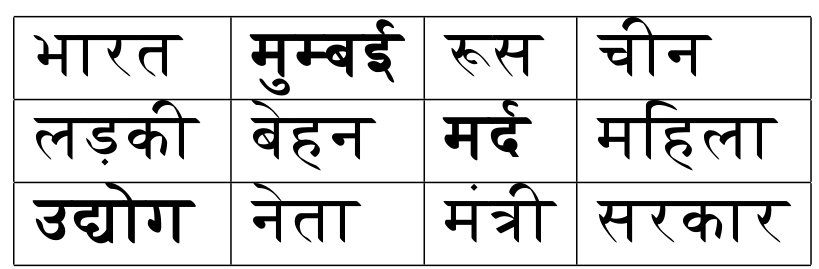
\includegraphics[scale=0.2]{odd_out.jpg}
\caption{Odd One Out in Hindi \label{fig:hindi_odd}}
\end{figure}
\vfill
}
%-------------------------------------slide---------------------------------
\frame{\frametitle{Similar Words}
\vfill
\begin{table}[ht!]
	\centering
	\begin{tabular}{|l|l|l|l|l|}
	\hline
	\textcolor{blue}{\textbf{Father}} & \textcolor{blue}{\textbf{France}} & \textcolor{blue}{\textbf{XBOX}} & \textcolor{blue}{\textbf{scratched}} & \textcolor{blue}{\textbf{megabits}} \\ \hline
	grandfather & Germany & XBLA  & scraped & gigabits  \\ \hline 
	uncle & French & Xbox360  & rubbed & kilobits  \\ \hline 
	mother & Greece & SmartGlass  & bruised & megabit  \\ \hline 
	father-in-law & Netherlands & 360/PS3  & cracked & terabits  \\ \hline 
	brother & Scotland & XBLA   & discarded & MB/s  \\ \hline 
	- & - & Qubed  & shoved & Tbit/s  \\ \hline 
	- & - & Kinect  & tripped & -  \\ \hline 
	\end{tabular}
	\caption{Top Few Similar words in English}
	\label{fig:english_similar}
\end{table}
\begin{figure}[ht!]
\centering
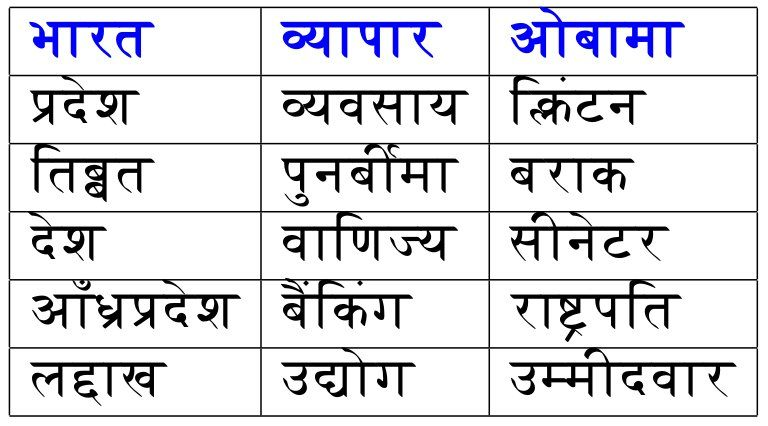
\includegraphics[scale=0.15]{similar_hindi.jpg}
\caption{Top Few Similar words in Hindi \label{fig:hindi_similar}}
\end{figure}
\vfill
}
%===========================================================================
\section[Conclusion and Future Work]{Conclusion and Future Work}
\subsection{}

%-------------------------------------slide---------------------------------
\frame{\frametitle{Conclusion}
  \begin{beamerboxesrounded}[shadow=true]{}
     \begin{enumerate}
		 \setlength\itemsep{1em}
		 \item<1-> We present a unsupervised language independent model that
		 \begin{itemize}
		 	\item<1-> overcomes the problems of BOW models
		 	\item<1-> gives individual importance to words as well as sentences as a whole
		 \end{itemize} 
		 \vfill\item<2-> We overcome the problems of language dependent models such as Recursive Tensor Neural Network(Socher et al., 2013)
		 \vfill\item<3-> We release a larger and more generic dataset of Hindi movie reviews 
		 \vfill\item<4-> We improve the state-of-the-art results on sentiment analysis
		 \begin{itemize}
		 	\item<4-> On the IMDB dataset, we improve by 1.6\%
		 	\item<4-> On the Amazon electronics dataset, we improve by 7.01\%
		 	\item<4-> On the Hindi product and movie reviews, we improve by 13.86\% and 11.30\% respectively
		 \end{itemize}
	\end{enumerate}
  \end{beamerboxesrounded}
}
%-------------------------------------slide---------------------------------
\frame{\frametitle{Future Work}
  \begin{beamerboxesrounded}[shadow=true]{}
	\begin{enumerate}
		 \setlength\itemsep{3em}
		 \item<1-> Better Composition Methods
		 \vfill\item<2-> Enhanced document vectors has given an indication that current representations are not sufficient to model documents and that ensembles could also prove useful in tasks such as sentiment analysis
		 \vfill\item<3-> \emph{Region of Importance} in NLP where we filter out sentiment oriented sentences and phrases from a unfocused corpus which contains text from various domains 
	\end{enumerate}
  \end{beamerboxesrounded}
}

%-------------------------------------slide---------------------------------
\frame{\frametitle{}
%  \begin{beamerboxesrounded}[shadow=true]{}
   %\centering{\Large{Questions?}}
    \begin{figure}
      \centering
      
\includegraphics[scale=0.2]{../img/questions.png}
    \end{figure}
%  \end{beamerboxesrounded}
}

%-------------------------------------slide---------------------------------
\frame{\frametitle{}
  \begin{beamerboxesrounded}[shadow=true]{}
   \centering{\Large{Thank you!}}
  \end{beamerboxesrounded}
}

%===========================================================================
\section[Appendix]{Appendix}
\subsection{}
%-------------------------------------slide---------------------------------
\frame{\frametitle{}
\textbf{Ensemble of RNNLM and Enhanced Document Vectors}\\
\begin{beamerboxesrounded}[shadow=true]{}
	\begin{itemize}
		 \item<1-> We first trained a \emph{recurrent neural network} and then obtained predictions on test reviews in terms of probability. 
		 \vfill\item<1-> We trained another classier(Linear SVM) using Enhanced Document Vectors and then obtained predictions on test reviews.
		 \vfill\item<1-> We then merged these two predictions using a simple heuristic, described below, to obtain final classification.
	\end{itemize}
  \end{beamerboxesrounded}
Let $y*$ be actual output and $y$ is the predicted output. The heuristic used is:
\begin{align*}
((RNNLM_{pred}-1)*7+(0.5-SVM_{pred})).y<0 \text{  if } y*=1\\
((RNNLM_{pred}-1)*7+(0.5-SVM_{pred})).y<0 \text{  otherwise}
\end{align*}
}
%-------------------------------------slide---------------------------------
\frame{\frametitle{}
\textbf{SkipGram}\\
$h=x^TW=v_{w_i}$\\
$v_{w_i}$ is the vector representation of the input word $w_i$\\
$u_j={v'}_{w_j}^T.h$\\
$u_j$ is score of each word in vocabulary and ${v'}_{w_j}$ is the $j-th$ column of matrix $W'$\\
$p(w_{c,j}=w_{O,c}|w_I)=y_{c,j}=\frac{exp(u_{c,j})}{\sum_{{j'}=1}^{V}exp(u_{j'})}$\\
where $w_{c,j}$ is the $j$-th word on the $c$-th panel of the output layer; $w_{O,c}$ is the actual $c$-th word in the output context words; $w_I$ is the only input word; $y_{c,j}$ is the output of the $j$-th node on the $c$-th panel of the output layer; $u_{c,j}$ is the net input of the $j$-th node on the $c$-th panel of the output layer.
}
%-------------------------------------slide---------------------------------
\frame{\frametitle{}
\textbf{SkipGram}\\
$u_{c,j}=u_j={v'}_{w_j}^T.h$, for $c=1,2,\dots,C$\\
Loss functions is:\\
$E=-log p(w_{O,1},w_{O,2},\dots,w_{O,C}|w_I)$\\
$=-log\prod_{c=1}^C\frac{exp(u_{c,{j*}_{c}})}{\sum_{{j'}=1}^Vexp({{u}_{j'}})}$
}
\end{document}
